%% Bookheader, Nov 8, 2020; July 18, 2022

\documentclass[11pt]{../Support/ourbook}
%% or for landscape, comment out line above and use this one:
%%\documentclass[landscape,11pt]{ourbook}

%% This will keep space from stretching around display math:

\makeatletter
\renewcommand\normalsize{%
   \@setfontsize\normalsize\@xipt{13.6}%
   \abovedisplayskip 11\p@  \@minus6\p@
   \abovedisplayshortskip \z@ 
   \belowdisplayshortskip 6.5\p@ \@minus3\p@
   \belowdisplayskip \abovedisplayskip
   \let\@listi\@listI}
\makeatother
\normalsize


\begin{document}

\tableofcontents
\graphicspath{{../../Chapters/matter_energy_intro/en_US}}
\chapter{Introduction to the Kontinua Sequence}

This book will start you on the long and difficult trek to becoming a modern
problem solver. Along the path, you will learn how to use the tools of
math, computers, and science. 

Why should you bother? There are big problems in this world that will
require expert problem solvers. Those people will make the world a
better place while enjoying interesting and lucrative careers. We are
talking about engineers, scientists, doctors, computer programmers,
architects, actuaries, and mathematicians. Right now, those occupations represent
about 6\% of all the jobs in the United States. Soon,
that number is expected to rise above 10\%.  On average, people in
that 10\% of the population are expected to have salaries twice that
of their non-technical counterparts.\index{career}

Solving problems is difficult. At some point on this journey, you will
see people who are better at solving problems than you are. You, like
every other person who has gone on this journey, will think ``I have
worked so hard on this, but that person is better at it than
I am. I should quit.'' Don't.\index{quitting}

First, solving problems is like a muscle. The more you do, the better
you get at it.  It is OK to say ``I am not good at this yet.'' That
just means you need more practice.

Second, you don't need to be the best in the world. 10 million people
your age can be better at solving problems than you, \textit{and you
  can still be in the top 10\% of the world}. If you complete this
journey, there will be problems for you to solve and a job where your
problem-solving skills will be appreciated.

So where do we start?

\section{Matter and Energy Introduction}

The famous physicist Richard Feynman once asked this question: ``If,
in some cataclysm, all of scientific knowledge were to be destroyed,
and only one sentence was passed on to the next generation of
creatures, what statement would contain the most information in the
fewest words?''

His answer was ``All things are made of atoms—little particles that move around in
perpetual motion, attracting each other when they are a little
distance apart, but repelling upon being squeezed into one another.''

That seems like a good place to start.\index{atom}

All things (including the air around you) are made of atoms. Atoms are
very tiny -- there are more atoms in a drop of water than there are
drops of water in all the oceans.
% ADD: If you want a better visual of the scale: https://htwins.net/scale2/, start at around 10^-8

Every atom has a nucleus that contains protons and neutrons. There is also
a cloud of electrons flying around the nucleus. However, the mass of the atom
comes mainly from the protons and neutrons, which are exponentially heavier
than electrons.\index{protons} \index{neutrons} \index{electrons}

\includegraphics[width=1\textwidth]{atom1.png}

Watch \textbf{Elements and atoms} from Khan Academy at \url{https://youtu.be/IFKnq9QM6_A}.

\subsection{Models of the Atom} 
Over the history of science, there have been many ideas about the structure of 
atoms. This history is a good example of how science develops: how unexpected 
results drive scientists to update their models, moving us closer and closer to 
a true model of the atom. During his investigations into the behavior of gases, 
John Dalton (lived 1766-1844) noted that different elements combine in strict 
ratios. For example, he noted that nitrogen and oxygen combine in a 1:1 and 1:2 
fashion, but no ratio in between.

This first model of the atom is very rudimentary: each element is a unique atom, 
and atoms cannot be subdivided. The atom is modeled as one large, solid, uniform, 
and neutral object. Some scientists, including the British physicist J.J. Thomson 
(1856-1940) thought that larger atoms (like lead) might be able to be broken down
into smaller atoms (like hydrogen). Thomson had been experimenting with cathode 
ray tubes and discovered that the these rays traveled much faster than thought 
possible for a particle the size of a hydrogen atom. This, combined with the 
observation that cathode rays could be deflected by electrical charge, led him to 
postulate two things:

\begin{enumerate}
\item atoms can be broken into parts much smaller than a hydrogen atom
\item whatever part of atoms that composes cathode rays is negatively charged
\end{enumerate}

The presence of "corpuscules" (as Thomson called them) that were negatively 
charged and smaller than a hydrogen atom contradicted Dalton's theory. Thomson 
updated his model of the atom: adding small, negatively charged subatomic 
particles (now called electrons) that were embedded in a larger, uniform, positive 
sphere. Suddenly, the atom went from neutral and indivisible to made of different 
types of charged particles. 

At the time, physicists were very interested in the mass-to-charge ratios of 
various particles (Thomson was able to determine the mass-to-charge ratio of the 
electron during his experiments), and Ernest Rutherford (1871-1937) was 
investigating the mass-to-charge ratio of alpha particles. (Alpha particles, we 
now know, are composed of two protons and two neutrons. They are emitted from 
certain radioactive elements, including uranium.) Rutherford needed consistent 
scattering of alpha particles in order to collect the data necessary to determine 
the particles' mass-to-charge ratio. He achieved this by bombarding extremely 
thin gold foil with alpha particles. The Thomson model of the atom would predict 
that particles would be slightly deflected, as illustrated below: 
FIXME insert thomson model scattering


However, a small but significant portion of the alpha particles were deflected 
over $90 \deg$! To explain this, Rutherford modeled the atom as mostly empty 
space with a small, dense, positive center (we now call this the nucleus).
FIXME rutherford model of the atom

At the same time that Rutherford was conducting his gold foil experiments, Niels 
Bohr was investigating the hydrogen line series FIXME insert figure of hydrogen 
lines. When hydrogen is electrically excited, it emits specific bands of color, 
not a complete spectrum. Bohr, upon learning of Rutherford's experiments, 
embraced the Rutherford model over the Thomson model and postulated that electrons 
existed only at discrete distances from the nucleus. When electrified, a hydrogen 
atom's electrons would gain energy and "jump" up one or more levels. The electron 
would be unstable in this energized state, and eventually "fall" back to the 
lowest energy level, emitting the extra energy as light. different colors of 
light have different energies: violet being the most energetic and red being the 
least. The different levels had differing amounts of energy between them, 
resulting in only those colors corresponding to the exact energy step between 
levels being emitted. This model, called the Bohr model or the Rutherford-Bohr 
model, expands on the Rutherford model by limiting electrons to specific 
distances from the nucleus, and is often compared to a model of the solar system 
FIXME add image of Bohr model. 

This is likely the model you are most familiar with seeing, and it is the one we 
will use often in this text. 


The previous graphic is slightly untrue. While it is a convenient model for 
thinking about atoms, in reality electrons don't neatly orbit the nucleus. 
Scientists don't know exactly where an electron will be in relation to the 
nucleus, but they do know where it's most likely to be. They use a cloud that is 
thicker in the center but fades out at the edges to represent an electron's 
position.


\includegraphics[width=.5\textwidth]{atomCloud.png}


We classify atoms by the numbers of protons they have. An atom with one proton is a
hydrogen atom, an atom with two protons is a helium atom, and so forth (refer to periodic table on pg..). We say that hydrogen and helium are \textit{elements} because the classification of elements is based on proton number. And we give
each element an atomic symbol. Hydrogen gets $H$. Helium gets $He$ Oxygen gets
$O$. Carbon gets $C$\index{elements}, etc.

Often two hydrogen atoms will attach to an oxygen atom. The result is
a water molecule. Why do they cluster together? because they share 
electrons in their clouds.\index{molecules}
% ADD:Electronegativity

A molecule is described by the elements it contains. Water is $H_2O$
because it has two hydrogen atoms and one oxygen atom.

There are many kinds of molecules. You know a few:
\begin{itemize}
\item Table salt is crystals made of $NaCl$ molecules: a sodium atom attached to a chlorine atom.
\item Baking soda, or sodium bicarbonate, is $NaHCO_3$.
\item Vinegar is a solution including acetic acid ($CH_3COOH$).
\item $O_2$ is the oxygen molecules that you breathe out of the air (Air, a blend of gases, is mostly $N_2$.).
\end{itemize}

\subsection{Reading the Periodic Table}
The Periodic Table organizes what we know about the structure of different 
elements. Each element has its own block or tile on the Periodic Table, and the 
information on the tile tells us about the structure of that atom. Take a look at 
the tile for carbon: (FIXME add carbon tile)

There are two key numbers: the atomic number and the average atomic mass. The 
atomic number tells how many protons there are in the nucleus of any atom of 
carbon. All carbon atoms have 6 protons. The other number is the average atomic 
mass. Have you heard of carbon-14 dating? The phrase "carbon-14" refers to a rare 
type of carbon that decays radioactively. By seeing how much carbon-14 has 
decayed, scientists can estimate the age of organic materials, such as bone or 
ash. Carbon-14 is a radioactive isotope (or version) of carbon. The 14 refers to 
the mass number - the total amount of protons AND neutrons in the nucleus. The 
most common isotope of carbon is carbon-12, with 6 protons and 6 neutrons in its 
nucleus. Carbon-14, on the other hand, has 8 neutrons, which makes the nucleus 
unstable, leading to radioactive decay. FIXME tow models comparing the structure 
of  C-12 and C-14. FIXME resource: atom builder PhET. The average atomic mass is 
the weighted average of all the carbon atoms in existence. Since the vast 
majority of carbon is carbon-12, the average atomic mass is very close to 12. You 
cannot determine the mass number of an individual atom from the periodic table: 
it only tells you the average of all the isotopes. However, especially for light 
atoms (atoms in the first two rows of the periodic table), you can usually 
determine the mass number of the most common isotope by rounding the average 
atomic mass to the nearest whole number. 

\section{Chemical Reaction}

Sometimes two hydrogen atoms form a molecule ($H_2$). Sometimes two
oxygen atoms form a molecule ($O_2$). If you mix these
together and light a match, they will rearrange themselves into water
molecules. This is called a \textit{chemical reaction}.  In any
chemical reaction, the atoms are rearranged into new molecules.\index{chemical reaction}
% ADD: electronegativity

Some chemical reactions (like the burning of hydrogen gas described
above) are \textit{exothermic} -- that is, they give off energy.
Burning hydrogen gas happens quickly and gives off a lot of energy. If
you have enough, it will make quite an explosion.\index{exothermic}
% ADD: endo/ exo thermic graphs/ explanation

\includegraphics[width=0.7\textwidth]{KA_Exo.png}

Other chemical reactions are \textit{endothermic} -- that is they consume
energy.  Photosynthesis, the process by which plants consume energy
from the sun to make sugar from $CO_2$ and $H_2O$ requires an endothermic
chemical reaction.\index{endothermic}

\includegraphics[width=0.7\textwidth]{KA_Endo.png}

In a chemical reaction, the transition state is the point where there is a maximum value of energy. This energy is called the activation energy. 

Here's an overview of chemical reactions: 
\url{https://simple.wikipedia.org/wiki/Chemical_reaction}


\section{Mass and Acceleration}

Each atom has a mass, so everything that is made up of atoms has a
mass, which is pretty much everything.  We measure mass in grams.  A
paper clip is about 1 gram of steel. An adult human can weigh 70,000
grams, so for larger things we often talk about kilograms. A kilogram
is 1000 grams.

The first interesting thing about mass is that objects with more mass
require more force to accelerate. For example, pushing a bicycle so
that it accelerates from a standstill to jogging speed in 2 seconds
requires a lot less force than pushing a train so that it accelerates
at the same rate.

You will probably find it useful to watch Khan Academy's summary of
Newton's second law of motion: \url{https://youtu.be/ou9YMWlJgkE}

\begin{mdframed}[style=important, frametitle={Newton's Second Law of Motion}]

The force necessary to accelerate an object of mass $m$ is given by:

$$F = m a$$

That is the force is equal to the mass times the acceleration.

\end{mdframed}

What are the units here? We already know that mass is measured in
kilograms. We can measure velocity in meters per second, but that is
different from acceleration. Acceleration is the rate of change in
velocity. So if we want to go from 0 to 5 meters per second (that's
jogging speed) in two seconds. That is a change in velocity of 2.5
meters per second every second. We would say this acceleration is $2.5
m/s^2$.

What about measuring force? Newton decided to name the unit after
himself: The force necessary to accelerate one kilogram at $1 m/s^2$
is known as \textit{a newton}.

\begin{Exercise}[title={Acceleration}, label=acceleration_train]
  
While driving a bulldozer, you come across a train car (with no brakes
and no locomotive) on a track in the middle of a city. The train car
has a label telling you that it weighs 2,400 kg. There is a bomb
welded to the interior of the train car, and the timer tells you that
you can safely push the train car for 120 seconds. To get the train
car to where it can explode safely, you need to accelerate it to 20 meters per
second. Fortunately, the track is level and the train car's wheels have
almost no rolling resistance.

With what force, in newtons, do you need to push the train for those 120 seconds?

\end{Exercise}
\begin{Answer}[ref=acceleration_train]
To get the train to 20 meters per second in 120 seconds, you must
accelerate it with a constant rate of $\frac{1}{6} m/s^2$. You
remember that $F = m a$, so $F = 2400 \times \frac{1}{6}$. Thus, you
will push the train with a force of 400 newtons for the 120 seconds
before the bomb goes off.
\end{Answer}

\section{Mass and Gravity}

The second interesting thing about mass is that masses are
attracted to each other by the force we call \textit{gravity}. The
force of attraction between two objects is proportional to the product
of their masses. As objects get farther away, the force decreases.
That is why you are more attracted to the earth than you are to
distant stars, which have much more mass than the earth.
%ADD: Collums Law

\begin{mdframed}[style=important, frametitle={Newton's Law of Universal Gravitation}]

Two masses ($m_1$ and $m_2$) that are a distance of
$r$ from each other, are attracted toward each other with a force of
magnitude:

$$F = G\frac{m_1 m_2}{r^2}$$

where $G$ is the universal gravitational constant. If you measure the
mass in kilograms and the distance in meters. $G$ is about $6.674
\times 10^{-11}$.  That will get you the force of the attraction in
newtons.

\end{mdframed}

\begin{Exercise}[title={Gravity}, label=gravity_earth]
  
  The earth's mass is about $6 \times 10^{24}$ kilograms.

  Your spacecraft's mass is 6,800 kilograms.

  Your spacecraft is also about 100,000 km from the center of the earth. (For reference, the moon is about 400,000 km from the center of the earth.)

  What is the force of gravity that is pulling your spacecraft and the earth toward each other?

\end{Exercise}
\begin{Answer}[ref=gravity_earth]

  $$F = G\frac{m_1 m_2}{r^2} = (6.674 \times 10^{-11})\frac{(6.8 \time 10^3)(6 \times 10^{24})}{(10^5)^2} = 6.1 \times 10^{6}$$

  About 6 million newtons.
  
\end{Answer}

\section{Mass and Weight}

Gravity pulls on things proportional to their mass, so we often
ignore the difference between mass and weight.

The weight of an object is the force due to the object's mass and
gravity.  When we say, ``This potato weighs 1 pound,'' we actually mean
``This potato weighs 1 pound on earth.''  That same potato would weigh
about one-fifth of a pound on the moon.

\includegraphics[width=1\textwidth]{massvweight.png}

But that potato has a mass of 0.45 kg anywhere in the universe.

FIXME Global layout note: Let's discuss adding Title's and Captions to all graphics.\\

For example:\\
TITLE: Mass versus Weight\\
CAPTION: Human Earth weight: 150lbs / Moon weight:??lbs\\
Potato Earth weight: .25lbs / Moon weight: ??lbs \\

FIXME: 
Allison thinks it would be funny if the person in the graphic were holding a potato and we also added the weight and mass of the  potato to the caption. No worries if this type of edit isn't in the budget! 

FIXME: What are your thoughts about using the metric system consistently -- in which case we'll replace pounds here with kilos. Max notes: we should explicitly use kilos for mass and pounds or newtons for weight. Kilos are a scalar measure of the amount of matter and pounds are a vector force of gravity on a particular piece of matter. Many students struggle to differentiate between mass and weight at a theoretical level due to casual comparison between pounds and kilos. 

\graphicspath{{../../Chapters/atomic_mass/en_US}}
\chapter{Introduction to the Kontinua Sequence}

This book will start you on the long and difficult trek to becoming a modern
problem solver. Along the path, you will learn how to use the tools of
math, computers, and science.

Why should you bother? There are big problems in this world that will
require expert problem solvers. Those people will make the world a
better place while enjoying interesting and lucrative careers. We are
talking about engineers, scientists, doctors, computer programmers,
architects, actuaries, and mathematicians. Right now, those occupations represent
about 6\% of all the jobs in the United States. Soon,
that number is expected to rise above 10\%.  On average, people in
that 10\% of the population are expected to have salaries twice that
of their non-technical counterparts.\index{career}

Solving problems is difficult. At some point on this journey, you will
see people who are better at solving problems than you are. You, like
every other person who has gone on this journey, will think ``I have
worked so hard on this, but that person is better at it than
I am. I should quit.'' Don't.\index{quitting}

First, solving problems is like a muscle. The more you do, the better
you get at it.  It is OK to say ``I am not good at this yet.'' That
just means you need more practice.

Second, you don't need to be the best in the world. 10 million people
your age can be better at solving problems than you, \textit{and you
  can still be in the top 10\% of the world}. If you complete this
journey, there will be problems for you to solve and a job where your
problem-solving skills will be appreciated.

\emph{Where do we start?}

The famous physicist Richard Feynman once asked this question: ``If,
in some cataclysm, all of scientific knowledge were to be destroyed,
and only one sentence was passed on to the next generation of
creatures, what statement would contain the most information in the
fewest words?''

His answer was ``All things are made of atoms—little particles that move around in
perpetual motion, attracting each other when they are a little
distance apart, but repelling upon being squeezed into one another.''

\emph{That} seems like a good place to start.

\graphicspath{{../../Chapters/work_energy/en_US}}
\chapter{Work and Energy}

In this chapter, we are going to talk about how engineers define work
and energy. It frequently takes force to get work done. Let's start with thinking about the relationship between force and energy. As we learned earlier, Force is measured in
newtons, and one newton is equal to the force necessary to accelerate one
kilogram at a rate of $1 m/s^2$.

When you lean on a wall, you are exerting a force on the wall, but you
aren't doing any work. On the other hand, if you push a car for a mile,
you are clearly doing work. Work, to an engineer, is the force you
apply to something, as well as the distance that it moves, in the direction
of the applied force. We measure work in \textit{joules}. A joule is one
newton of force over one meter.\index{Joule}

\includegraphics[width=0.6\textwidth]{workvsforce.png}

For example, if you push a car uphill with a force of 10 newtons for 12
meters, you have done 120 joules of work.\index{work}
% ADD: We can represent this with the equations, Work Energy Therom

Work is how energy is transferred from one thing to another. When you
push the car, you also burn sugars(energy of the body) in your blood. That energy is then
transferred to the car: after it has been pushed uphill.

Thus, we measure the energy something consumes or generates in
units of work: joules, kilowatt-hours, horsepower-hours, foot-pounds,
BTUs( British Thermal Unit), and calories.

Let's go over a few different forms that energy can take.

\section{Forms of Energy}\index{energy!Forms of}

In this section we are going to learn about several different types of energy:
\begin{itemize}
\item Heat
\item Chemical Energy
\item Kinetic Energy
\item Gravitational Potential Energy
\end{itemize}

\subsection{Heat}\index{heat}

When you heat something, you are transferring energy to it. The BTU
 is a common unit for heat: One BTU is the
amount of heat required to raise the temperature of one pound of water,
by one degree. One BTU is about 1,055 joules. In fact, when you buy and sell
natural gas as fuel, it is priced by the BTU.\index{heat} \index{BTU}

\subsection{Electricity}\index{electricity}

Electricity is the movement of electrons. When you push electrons
through a space that resists their passage (like a light bulb),
energy is transferred from the power source ( a battery)
 into the source of the resistance.

Let's say your lightbulb consumes 60 watts of electricity, and you leave it on for 24 hours.
We would say that you have consumed 1.44 kilowatt hours or 3,600,000 joules.


\subsection{Chemical Energy}\index{chemical energy}

As mentioned early, some chemical reactions consume energy and some
produce energy. Thus, energy can be stored in the structure of a
molecule. When a plant uses photosynthesis to rearrange water and
carbon dioxide into a sugar molecule, it converts the energy in
the sunlight( solar energy) into chemical energy. Remember photosythesis is a process that releases energy.
Therefore, the sugar molecule has more chemical energy than the carbon dioxide and water molecules that were
used in its creation.
% ADD: photosythesis equation
% KA: https://www.khanacademy.org/science/ap-biology/cellular-energetics/photosynthesis/a/intro-to-photosynthesis

In our diet, we measure this energy in \textit{kilocalories}. A
calorie is the energy necessary to raise one gram of water one degree
Celsius: it is about 4.19 joules. This is a very small unit: an apple
has about 100,000 calories( 100 kilocalories), so people working with food started
measuring everything in kilocalories.\index{calories}
% ADD: Conversion chapter should come before this chapter

Here is where things get confusing: People who work with food got tired of
saying ``kilocalories'', so they just started using ``Calorie'' to
mean 1,000 calories.  This has created terrible confusion over the
years. So if the C is capitalized, ``Calorie'' probably means kilocalorie.

\subsection{Kinetic Energy}\index{kinetic energy}

A mass in motion has energy. For example, if you are in a moving car
and you slam on the breaks, the energy from the motion of the
car will be converted into heat in the breaks and under the tires.

How much energy does the car have?
% ADD: section specifically about KE AND U, use roller coaster diagram

\begin{mdframed}[style=important, frametitle={Formula for Kinetic Energy}]

$$E = \frac{1}{2} m v^2$$

where $E$ is the energy in joules, $m$ is the mass in kilograms, and
$v$ is the speed in meters per second.

\end{mdframed}

\subsection{Gravitational Potential Energy}\index{potential energy!gravitational}


When you lift something heavy onto a shelf, you are giving it
\textit{potential energy}. The amount of energy that you transferred
to it is proportional to its weight and the height that you lifted it.

On the surface of the earth, gravity will accelerate a heavy object downward at
a rate of $9.8 m/s^2$.

\begin{mdframed}[style=important, frametitle={Formula for Gravitational Potential Energy}]
The formula for gravitational potentional energy is

$$E = mgh$$

where $E$ is the energy in joules, $m$ is the mass of the object you
lifted, $g$ is acceleration due to gravity, and $h$ is the height that you lifted it.

On earth, then, gravitational potential energy is given by

$$E = (9.8)mh$$

since objects accelerate at $9.8 m/s^2$.

\end{mdframed}


There are other kinds of potential energy. For example, when you draw
a bow, you have given that bow potential energy. When you release it,
the potential energy is transferred to the arrow, which expresses it
as kinetic energy.
% ADD: section about KE and U

\section{Conservation of Energy}

The first law of thermodynamics says ``Energy is neither created nor
destroyed.''\index{energy!conservation of}

Energy can change forms: Your cells consume chemical energy to give
gravitational potential energy to a car you push up a hill. However, the total amount of
energy in a closed system stays constant.
% ADD: Create Systems chapter before introducing concept here

\begin{Exercise}[title={The Energy of Falling}, label=energy_falling]

A 5 kg cannonball falls off the top of a 3 meter ladder. As it falls,
its gravitational potential energy is converted into kinetic energy.
How fast is the cannonball traveling just before
it hits the floor?

\end{Exercise}
\begin{Answer}[ref=energy_falling]

  At the top of the ladder, the cannonball has $(9.8)(5)(3) = 147$ joules of potential energy.

  At the bottom, the kinetic energy $\frac{1}{2}(5)v^2$ must be equal
  to 147 joules. So $v^2 = \frac{294}{5}$.  Thus it is going about
  $7.7$ meters per second.

  (Yes, a tiny amount of energy is lost to air resistance. For a dense
  object moving at these relatively slow speeds, this energy is
  neglible.)

\end{Answer}


\section{Efficiency}



Although energy is always conserved as it moves through different
forms, scientists aren't always that good at controlling it.\index{efficiency}

For example, a car engine consumes the chemical energy in gasoline. Only
about 20\% of the energy consumed is used to turn the wheels.  Most of
the energy is actually lost as heat. If you run a car for a while, the engine
gets very hot and the exhaust going out the tailpipe turns hot.

A human is about 25\% efficient. Most of the loss is in the heat produced
during the chemical reactions that turns food into motion.
% ADD: Cellular Respiration

In general, if you are trying to increase efficiency in any system,
the solution is usually easy to identify because heat is produced. Reduce heat, Increase efficiency.

Light bulbs are an interesting case. To get the light of a 60 watt
incandescent bulb, you can use an 8 watt LED or a 16 watt fluorescent
light. Thus, we say that the LED light is much more efficient: If you
run both, the incandescent bulb will consume 1.44 kilowatt-hours. The
LED will consume only 0.192 kilowatt-hours.

Besides light, the incandescent bulb is producing a lot of heat. If it
is inside your house, what happens to the heat? It warms your house.

In the winter, when you want light and heat, the incandescent bulb is
100\% efficient!

In the summer, if you are running the air conditioner, the
incandescent bulb is worse than just ``inefficient at making light'' --
it is actually counteracting the air conditioner!

\graphicspath{{../../Chapters/units_conversions/en_US}}
\chapter{Introduction to the Kontinua Sequence}

This book will start you on the long and difficult trek to becoming a modern
problem solver. Along the path, you will learn how to use the tools of
math, computers, and science.

Why should you bother? There are big problems in this world that will
require expert problem solvers. Those people will make the world a
better place while enjoying interesting and lucrative careers. We are
talking about engineers, scientists, doctors, computer programmers,
architects, actuaries, and mathematicians. Right now, those occupations represent
about 6\% of all the jobs in the United States. Soon,
that number is expected to rise above 10\%.  On average, people in
that 10\% of the population are expected to have salaries twice that
of their non-technical counterparts.\index{career}

Solving problems is difficult. At some point on this journey, you will
see people who are better at solving problems than you are. You, like
every other person who has gone on this journey, will think ``I have
worked so hard on this, but that person is better at it than
I am. I should quit.'' Don't.\index{quitting}

First, solving problems is like a muscle. The more you do, the better
you get at it.  It is OK to say ``I am not good at this yet.'' That
just means you need more practice.

Second, you don't need to be the best in the world. 10 million people
your age can be better at solving problems than you, \textit{and you
  can still be in the top 10\% of the world}. If you complete this
journey, there will be problems for you to solve and a job where your
problem-solving skills will be appreciated.

\emph{Where do we start?}

The famous physicist Richard Feynman once asked this question: ``If,
in some cataclysm, all of scientific knowledge were to be destroyed,
and only one sentence was passed on to the next generation of
creatures, what statement would contain the most information in the
fewest words?''

His answer was ``All things are made of atoms—little particles that move around in
perpetual motion, attracting each other when they are a little
distance apart, but repelling upon being squeezed into one another.''

\emph{That} seems like a good place to start.

\graphicspath{{../../Chapters/simple_machines/en_US}}
\chapter{Simple Machines}

As mentioned earlier, physicists define work as the force applied times the distance over which it is applied. For example, if you push your car 100 meters with a force of 17 newtons, you have done 1700 joules of work.

Humans have long needed to move heavy objects, so many centuries ago, we developed simple machines to reduce the amount of force necessary to perform such tasks. These include:

\begin{itemize}
    \item Levers
    \item Pulleys
    \item Inclined planes
    \item Gears
    \item Hydraulics
    \item Screws
\end{itemize}

\includegraphics[width=\textwidth]{simplemachines.png}

While these machines can reduce the force needed, they do not change the total amount of work that must be done. For instance, if the force is reduced by a factor of three, the distance over which the force must be applied increases by the same factor.

The term \textit{mechanical advantage} refers to the increase in force achieved by using these machines.

\section{Levers}

A lever pivots on a fulcrum. To decrease the necessary force, the load is placed closer to the fulcrum than where the force is applied.

Physicists also discuss the concept of \newterm{torque} created by a force. When you apply force to a lever, the torque is the product of the force you exert and the distance from the point of rotation.

Torque is typically measured in newton-meters.

To balance two torques, the products of force and distance must be equal. Thus, assuming the forces are applied in the correct direction, the equation becomes:

\[
R_L F_L = R_A F_A
\]

where \( R_L \) and \( R_A \) represent the distances from the fulcrum to where the load’s force and the applied force are exerted, respectively, and \( F_L \) and \( F_A \) are the magnitudes of the forces.

\begin{Exercise}[title={Lever}, label=lever]
Paul, who weighs 70 kilograms, sits on a see-saw 4 meters from the fulcrum. Jan, who weighs 50 kilograms, wishes to balance the see-saw. How far should Jan sit from the fulcrum?
\end{Exercise}
\begin{Answer}[ref=lever]
Paul exerts a force of \( 70 \times 9.8 = 686 \) newtons at a distance of 4 meters from the fulcrum, creating a torque of \( 686 \times 4 = 2744 \) newton-meters. Jan exerts a force of \( 50 \times 9.8 = 490 \) newtons.

Let \( r \) be the distance from the fulcrum to Jan's seat. To balance the torques:

\[
490 \times r = 2744
\]

Solving for \( r \), we find \( r = \frac{2744}{490} \approx 5.6 \) meters.
\end{Answer}

\includegraphics[width=0.6\textwidth]{seesaw.png}

\section{Inclined Planes}

Inclined planes, or ramps, allow you to roll or slide objects to a higher level. Steeper ramps require less mechanical advantage. For instance, it is much easier to roll a ball up a wheelchair ramp than a skateboard ramp.

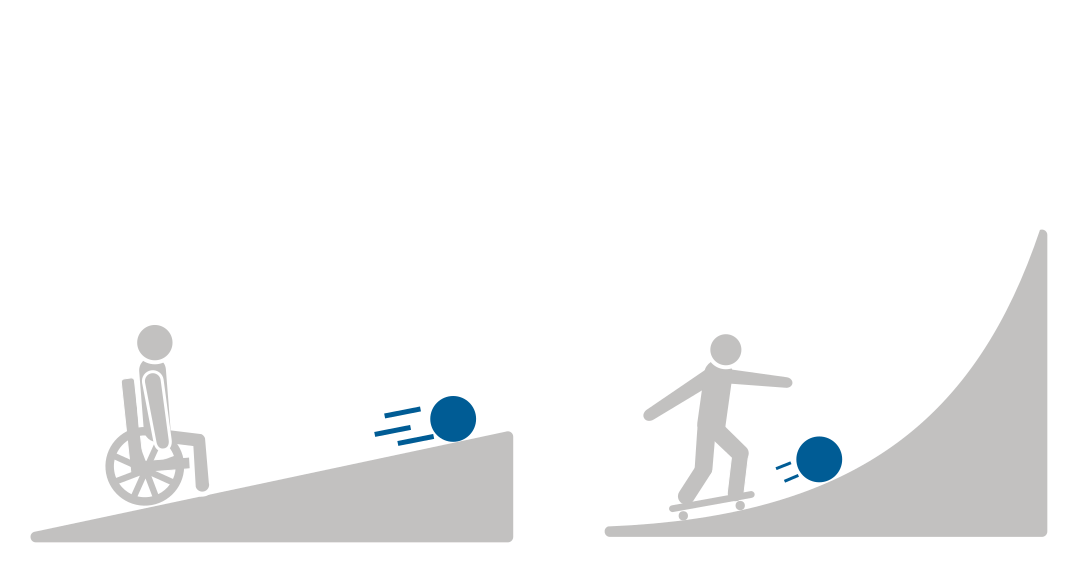
\includegraphics[width=\textwidth]{rampcomparison.png}

Assuming the incline has a constant steepness, the mechanical advantage is equal to the ratio of the length of the inclined plane to the height it rises.

If friction is neglected, the force required to push a weight up the inclined plane is given by:

\[
F_A = \frac{V}{L} F_G
\]

where \( F_A \) is the applied force, \( L \) is the length of the inclined plane, \( V \) is the vertical rise, and \( F_G \) is the gravitational force acting on the mass.

(We haven't yet discussed the sine function, but in case you're familiar with it, note that:

\[
\frac{V}{L} = \sin{\theta}
\]

where \( \theta \) is the angle between the inclined plane and the horizontal surface.)

\begin{Exercise}[title={Ramp}, label=ramp]
A barrel of oil weighs 136 kilograms. You can apply a force of up to 300 newtons. You need to get the barrel onto a platform that is 2 meters high. What is the shortest length of inclined plane you can use?
\end{Exercise}
\begin{Answer}[ref=ramp]
The weight of the barrel is \( 136 \times 9.8 = 1332.8 \) newtons.

Let \( L \) be the length of the inclined plane. The force needed to push the barrel up is related by:

\[
300 = \frac{2}{L} \times 1332.8
\]

Solving for \( L \), we find \( L = \frac{2 \times 1332.8}{300} \approx 8.885 \) meters.
\end{Answer}

\section{Gears}

Gears have teeth that mesh with each other. When you apply torque to one gear, it transfers torque to the other. The resulting torque is increased or decreased depending on the ratio of the number of teeth on the gears.

\includegraphics[width=0.7\textwidth]{gearsNew.png}

If \( N_A \) is the number of teeth on the gear you are turning with a torque of \( T_A \), and \( N_L \) is the number of teeth on the gear it is turning, the resulting torque is:

\[
T_L = \frac{N_A}{N_L} T_A
\]

\begin{Exercise}[title={Gears}, label=gear]
In a bicycle, the goal is not always to gain mechanical advantage, but to spin the pedals slower while applying more force.

You like to pedal your bike at 70 revolutions per minute. The chainring connected to your pedals has 53 teeth. The circumference of your tire is 2.2 meters. You want to ride at 583 meters per minute.

How many teeth should the rear sprocket have?
\end{Exercise}
\begin{Answer}[ref=gear]
The equation relating these quantities is:

\[
583 = 70 \times 2.2 \times \frac{53}{n}
\]

Solving for \( n \), we find \( n = 14 \) teeth.
\end{Answer}

\section{Hydraulics}

In a hydraulic system, such as a car's braking system, you exert force on a piston filled with fluid. The fluid transmits this pressure into another cylinder, where it pushes yet another piston that moves the load.

\includegraphics[width=\textwidth]{hydraulicsNew.png}

The pressure in the fluid is typically measured in pascals (Pa), which is equivalent to \(N / m^2\). We will use pascals for this calculation.

To calculate the pressure you create, divide the force applied by the area of the piston head. To determine the force on the other piston, multiply the pressure by the area of the second piston.

\begin{Exercise}[title={Hydraulics}, label=hydraulics]
Your car has disc brakes. When you apply 2,500,000 pascals of pressure to the brake fluid, the car stops quickly. As the car designer, you want this to require only 12 newtons of force from the driver's foot.

What should the radius of the master cylinder (the piston the driver pushes) be?
\end{Exercise}
\begin{Answer}[ref=hydraulics]
We are solving for the radius \( r \) of the piston. The area of the piston is \( \pi r^2 \), so the pressure is:

\[
\text{Pressure} = \frac{12}{\pi r^2}
\]

Setting the pressure equal to 2,500,000 pascals:

\[
2,500,000 = \frac{12}{\pi r^2}
\]

Solving for \( r \), we find:

\[
r = \sqrt{\frac{12}{\pi \times 2.5 \times 10^6}} \approx 0.00124 \text{ meters}.
\]
\end{Answer}

\graphicspath{{../../Chapters/buoyancy/en_US}}
\chapter{Buoyancy}

The word buoyancy probably brings to mind images of floating in water. Before we dive in, let's zoom out for a moment and consider that the study of buoyancy is about much more than just boats and water. You might be thinking: I want to be a computer programmer, why do I need to know about buoyancy? This topic is much bigger than it might seem at first glance. Buoyancy concerns how all liquids and gasses interact with gravity. The concept of buoyancy is connected to fundamental concepts about how things work in the universe. The \newterm{buoyant force}, as it’s known in engineering, is an important concept that has wide ranging applications. A big part of engineering is moving stuff around, and understanding buoyancy helps us solve problems where we need to move things in and through fluids. Even if you don't have plans to build a robotic submarine, these are super useful ideas to be familiar with. We’ll start exploring the topic with familiar scenarios around boats and water.

When you put a boat into water, it will sink into the water until
the mass of the water it displaces is equal to the mass of the
boat. We think of this in terms of forces. Gravity pulls the mass of
the boat down. The \newterm{buoyant force} pushes the boat up. A boat
dropped into the water will bob up and down a bit before reaching an
\newterm{equilibrium} where the two forces are equal.
% ADD: Explain Action Reaction Pairs in previous chapter
% ADD: Archimedes principle

The buoyant force pushes things up -- against the force of
gravity. The force is equal to the weight of the fluid being
replaced. So, for example, a cubic meter of freshwater has a mass of
about 1000kg.  If you submerge anything with a volume of one meter in
freshwater on earth, the buoyant force will be about 9800 newtons.

For some things, like a block of styrofoam, this buoyant force will be
sufficient to carry it to the surface. Once it reaches the surface, it
will continue to rise (displacing less water) until the mass of the
water it displaces is equal to its mass. And then we say ``It floats!''

\includegraphics[width=.6\textwidth]{waterDisplacement.png}

For some things, like a block of lead, the buoyant force is not
 sufficient to lift it to the surface, and thus we say ``It sinks!''

This is why a helium balloon floats through the air. The air
that it displaces weighs more than the balloon and the helium itself. (It is easy to forget that air has a mass, but it does.)

\begin{Exercise}[title={Buoyancy}, label=buoyancy]
  You have an aluminum box that has a heavy base, so it will always
  float upright. The box and its contents weigh 10 kg. Its base is 0.3 m x 0.4 m. It is 1m tall.

  When you drop it into freshwater ($1000 kg/m^3$), how far will it sink
  before it reaches equilibrium.\index{equilibrium}

\end{Exercise}
\begin{Answer}[ref=buoyancy]
  Equilibrium will be achieved when the box has displaced 10 kg of water. That is, when it has displaced $0.01$ cubic meters.

  The area of the base of the box is 0.12 square meters.  So if the
  box sinks $x$ meters into the water it will displace $0.12 x$ cubic
  meters.

  Thus at equilibrium $x = \frac{0.01}{0.12} \approx 0.083$ m.  So,
  the box will sink 8.3 cm into the water before reaching equilibrium.
\end{Answer}

\section{The Mechanism of Buoyancy: Pressure}

As you dive down in the ocean, you will experience greater and
greater pressure from the water. And if you take a balloon with you, you
will gradually see it get smaller as the water pressure compresses the
air in the balloon.

Let's say you are 3 meters below the surface of the water. What is the
pressure in Pascals (newtons per square meter)? You can think of the
water as a column of water crushing down upon you. The pressure over
a square meter is the weight of 3 cubic meters of water pressing down.

$$p = (3)(1000)(9.8) = 29,400 \text{ Pa }$$

This is called \newterm{hydrostatic pressure}. The general rule for
hydrostatic pressure in Pascals $p$ is

$p = d g h$

Where  $d$ is the density of the fluid
in kg per cubic meter, $g$ is the acceleration due to gravity in
$m/s^2$, and $h$ is the height of the column of fluid above you.

So, where does buoyant force come from? Basically, the pressure pushing up on the
deepest part of the object is higher than the pressure pushing down on
the shallowest part of the object. That is where bouyancy comes from.

\includegraphics[width=.6\textwidth]{buoyancy.png}

\begin{Exercise}[title={Hydrostatic Pressure}, label=mars_pressure]

  You dive into a tank of olive oil on Mars. How much more
  hydrostatic pressure does your body experience at 5 meters deep than
  it did at the surface?

  The density of olive oil is about 900 kg per square meter. The
  acceleration due to gravity on Mars is 3.721 $m/s^2$.

\end{Exercise}
\begin{Answer}[ref=mars_pressure]
$$p = d g h = (900)(3.721)(5) = 16,744.5 \text{ Pa}$$
\end{Answer}

\section{The Mechanism of Buoyancy: Density}
Notice that although the pressure is increasing as you go deeper, the
buoyant force will \emph{not increase} because the buoyant force is always equal
to the weight of the fluid that is displaced, regardless if that is 1
meter or 100 meters underwater.

Due to the added minerals, saltwater is denser than freshwater. This causes objects float
better in the sea than they do in, say, a river. Lipids, like fats and
oils, are less dense than water, allowing them to float on top of a glass of water.
When you're facing a grease fire, you're told not to put water on it. That's because
the water sinks below the grease, then boils, throwing burning grease everywhere.

\graphicspath{{../../Chapters/heat/en_US}}
\chapter{Introduction to the Kontinua Sequence}

This book will start you on the long and difficult trek to becoming a modern
problem solver. Along the path, you will learn how to use the tools of
math, computers, and science.

Why should you bother? There are big problems in this world that will
require expert problem solvers. Those people will make the world a
better place while enjoying interesting and lucrative careers. We are
talking about engineers, scientists, doctors, computer programmers,
architects, actuaries, and mathematicians. Right now, those occupations represent
about 6\% of all the jobs in the United States. Soon,
that number is expected to rise above 10\%.  On average, people in
that 10\% of the population are expected to have salaries twice that
of their non-technical counterparts.\index{career}

Solving problems is difficult. At some point on this journey, you will
see people who are better at solving problems than you are. You, like
every other person who has gone on this journey, will think ``I have
worked so hard on this, but that person is better at it than
I am. I should quit.'' Don't.\index{quitting}

First, solving problems is like a muscle. The more you do, the better
you get at it.  It is OK to say ``I am not good at this yet.'' That
just means you need more practice.

Second, you don't need to be the best in the world. 10 million people
your age can be better at solving problems than you, \textit{and you
  can still be in the top 10\% of the world}. If you complete this
journey, there will be problems for you to solve and a job where your
problem-solving skills will be appreciated.

\emph{Where do we start?}

The famous physicist Richard Feynman once asked this question: ``If,
in some cataclysm, all of scientific knowledge were to be destroyed,
and only one sentence was passed on to the next generation of
creatures, what statement would contain the most information in the
fewest words?''

His answer was ``All things are made of atoms—little particles that move around in
perpetual motion, attracting each other when they are a little
distance apart, but repelling upon being squeezed into one another.''

\emph{That} seems like a good place to start.

%%%%%%%%%%%%%%%%%%%%%%%%%%%%%%%%%
%% Bookfooter.tex by Aaron Hillegass
%% Nov 8, 2020

\appendix

\chapter{Answers to Exercises}
\shipoutAnswer

\bibliography{references}

\printindex

\end{document}